\label{chapter:Resultados}

\par
\textcolor{red}{Nesta seção serão apresentados os resultados obtidos após as avaliações do modelo, que foi feito com os algoritmos de classificação e associação. Será demonstrado quais variáveis foram classificadas com maior relevância, as ramificações geradas com maior quantidade de registros que percorrem elas, além das regras obtidas para base através do algoritmo de associação.}

\section{Classificação}

\par
\textcolor{red}{Os resultados obtidos com o algoritmo de classificação apresentam um valor mediano de acurácia para o modelo utilizado. A técnica de classificação que foi utilizada, classificou corretamente em torno de 53\% das instâncias que pertence ao conjunto de teste, em relação à classe do resultado que foi obtido. Com base do modelo de árvore de decisão deduzido pelo algoritmo J48, foi possível analisar o grau de interação e a relação das variáveis de acordo com o caminho de interações percorrido pelas respostas do questionário feitas pelos candidatos.}

\par
\textcolor{red}{A árvore obtida apresentou como variável independente principal para a classificação o atributo Deficiencia, que se divide em 5 valores: Nao, Sim visual, Sim outro tipo, Sim fisica e Sim auditiva. As próximas variáveis com maior relevância mudavam de acordo com o valor que era obtido, sendo que, quando a resposta do candidato era de que ele não possuía alguma deficiência ou que ele possuía uma deficiência visual, a variável com maior importância para onde os valores eram direcionados era se ele frequentava ou frequenta cursinho particular, enquanto, para aqueles que possuíam deficiência física ou auditiva eram direcionados para a variável Cor (cor de pele), como apresentada na Figura 37.}

\par
\begin{figure}[!htp]
	\begin{center}
    \caption{\label{fig:waveform_fig} Representação das principais variáveis da árvore de decisão.}
	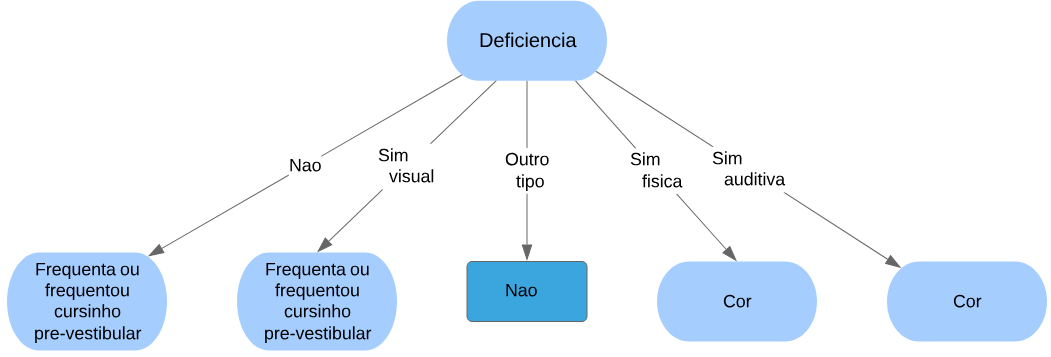
\includegraphics[scale=0.57]{Figuras/Arvore_gerada_grau2.png}
	\end{center}
    \legend{Fonte: Próprio autor.}
\end{figure}


\par
\textcolor{red}{É possível observar na Figura 37, que para os candidatos que responderam que possuíam outro tipo de deficiência, o valor da resposta era direcionado para um nó folha da classe Nao pertencente a variável dependente Aprovado, isto é, os candidatos que possuíam outro tipo de deficiência que não foram mencionados como opção de resposta da questão, não foram capazes de passar no vestibular (um total de 9 candidatos). A partir do terceiro nível de profundidade, para os candidatos que não possuíam nenhum tipo de deficiência a ramificação da árvore se expandia (tracejado pela linha vermelha), enquanto, diferentemente para os candidatos que possuíam algum tipo de deficiência, eles eram direcionados para os nós folhas da variável Aprovado (tracejado pela linha verde), como apresentado na Figura 38.}

\par
\begin{figure}[!htp]
	\begin{center}
    \caption{\label{fig:waveform_fig} Árvore completa.}
	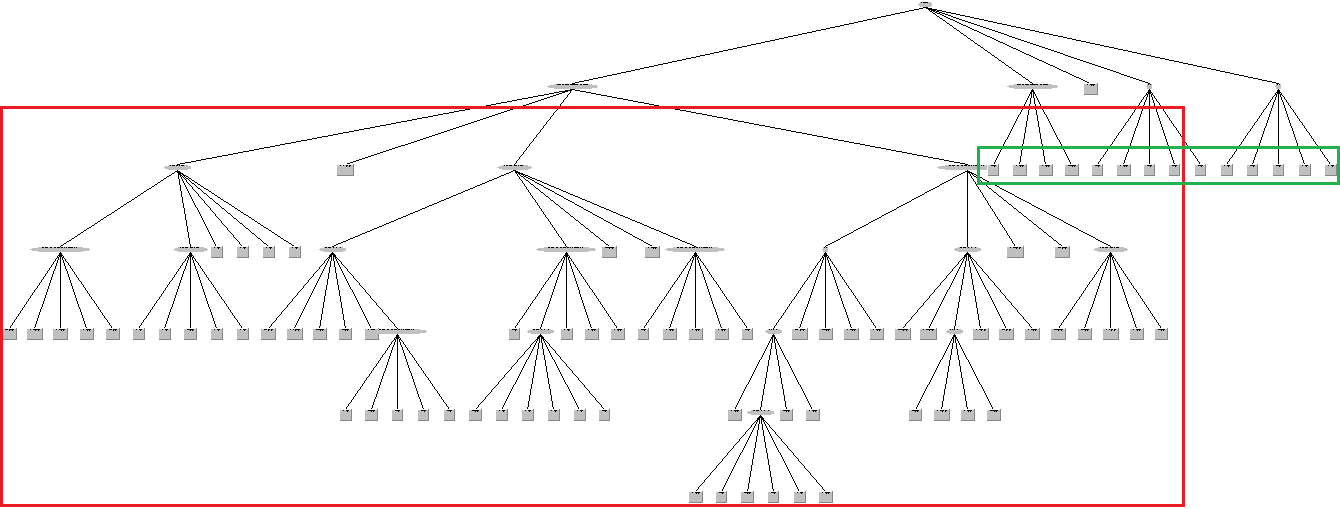
\includegraphics[scale=0.45]{Figuras/Arvore_completa.png}
	\end{center}
    \legend{Fonte: Próprio autor.}
\end{figure}


\subsection{Resultados obtidos para os candidatos que não possuiam nenhum tipo de deficiência}


\par
\textcolor{red}{Avaliando a árvore que foi gerada, através da maior quantidade de registros que se encaixam pelo caminho percorrido das ramificações até as folhas, foi obtido os seguintes resultados, começando pela ramificação maior que era a dos candidatos que não possuiam nenhum tipo de deficiencia, a variavel com maior relevancia que foi classificada após o variavel independente principal era se o candidato frequentava um cursinho pré-vestibular. Foi classificado que todos aqueles que frequentaram por mais de um ano algum cursinho, não foram aprovados no vestibular.}

\par
\textcolor{red}{Para aqueles que frequentaram o cursinho por um ano, o atributo correspondente seguinte era a quantidade de pessoas que moravam com ele, sendo que, a maior taxa de candidatos aprovados para essa variavel era quando possuia 3 pessoas morando com ele e para reprovados era quando possuia de 4 a 5 pessoas. Já para os candidatos que ficavam por um semestre fazendo o cursinho, a variavel correspondente seguinte era o meio de transporte que ele utilizava, a maior taxa de aprovados era pra aqueles que usavam o transporte coletivo e para os reprovados eram os outros tipos de transportes não eram mencionados como opção de resposta.}

\par
\textcolor{red}{Para aqueles que não frequentavam algum cursinho pré-vestibular, a variável classificada com maior relevância, seguinte, era a quantidade de pessoas que moravam com o candidato, e dependendo dos valores que eram respondidos para essa variável, os atributos em sequência variavam entre cor de pele, ocupação do pai e meio de transporte utilizado. Foi notado que as maiores taxas de aprovados eram para os candidatos pardos, que moravam de 3 a 5 pessoas e que o pai era servidor público, já para aqueles que não foram aprovados, as maiores taxas eram quando o candidato possuía de quatro ou mais pessoas morando com ele, o pai possuía outro tipo de ocupação e o meio de transporte utilizado era o coletivo.}


\subsection{Resultados obtidos para os candidatos que possuiam algum tipo de deficiência}


\par
\textcolor{red}{Diferente dos valores classificados para os candidatos que não possuíam algum tipo de deficiência, para aqueles que possuíam, o nível de profundidade que a ramificação delas alcançou não foi tão grande quanto a outra. Os resultados obtidos foram, primeiro, para os candidatos que eram deficientes visuais, a taxa de maior aprovação na prova era para aqueles que não frequentaram cursinho pré-vestibular, enquanto para aqueles que frequentaram cursinho por mais de um ano a taxa de reprovação era maior.}

\par
\textcolor{red}{Foi possível observar que tanto para os candidatos com deficiência física quanto para auditiva, a variável que mais influenciava para que eles fossem aprovados ou não era cor de pele. Sendo que para os candidatos com deficiência física, aqueles que eram brancos a chance de ser aprovado era maior, diferente para aqueles que eram pardos tendo sua taxa de reprovação muito alta comparada a outros tons de pele.}

\par
\textcolor{red}{Para os candidatos que possuíam deficiência auditiva, aqueles que tinham um tom de pele pardo obtiveram as maiores taxas de aprovação, ao contrário daqueles que possuíam uma cor de pele branca, a taxa de reprovação era alta. Como já foi mencionado anteriormente na parte de avaliação do trabalho, os candidatos que possuíam qualquer outro tipo de deficiência, foram classificados, que nenhum deles tiveram êxito de serem aprovados no vestibular.}


\section{Associação}

\textcolor{red}{Através dos resultados obtidos com o algoritmo de associação, observou que a medida que o suporte mínimo decrescia, a quantidade de regras que eram geradas aumentava. Os resultados das regras geradas foram divididos em duas partes, para os candidatos aprovados e para os candidatos não aprovados.}

%\textcolor{red}{787 registros aprovados, 7784 registros não aprovados, 8571.}


\subsection{Regras geradas para os candidatos aprovados}

\par
\textcolor{red}{Analisando as regras geradas em cada teste, na Tabela 3 que apresenta a tabela das regras gerada utilizando 22 atributos com 50\% de suporte, são interpretados da seguinte maneira. Para regra com menor transição de itens, diz que se o candidato possui outro tipo de trabalho não mencionado e a sua residência é própria então ele terá chance de ser aprovado com 100\% de confiança. Já para a maior regra gerada, diz que se o candidato não possui alguma deficiência, seu ensino médio é todo em escola pública e possui outro tipo de trabalho não mencionado, então a chance de ele passar é de 100\% de confiança. Para ambas as regras, acontece com 5\% dos candidatos (394 instancias).}


\par
\begin{table}[!htp]
	\begin{center}
    \caption{\label{fig:waveform_fig} Suporte Mínimo 50\% e Confiança Mínima 70\%.}
	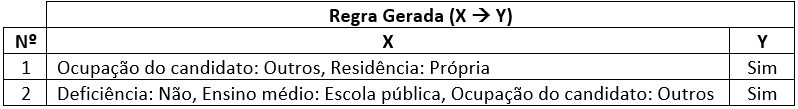
\includegraphics[scale=0.75]{Figuras/Suporte_50_atributos_22.png}
	\end{center}
\end{table}

\par
\textcolor{red}{Para os outros testes com 4 e 9 atributos, com a taxa de 50\% de suporte, nenhuma regra foi gerada para elas. Assim como os resultados do teste de 50\% de suporte, para os testes de 30\% das transições feitas com a quantidade de 4 e 9 atributos, nenhuma regra foi gerada também, já para a base com 22 atributos, foram geradas pelo menos 11 regras no geral, associadas com a variável Aprovados. Sendo que a primeira regra gerada possui 5 itens em sua transição e a última regra gerada chega a possuir 7 itens em sua transição. As regras foram geradas para 236 instancias (3\% dos candidatos), como apresentado na Tabela 4, onde é demonstrado a primeira e a ultima regra gerada.}

\par
\begin{table}[!htp]
	\begin{center}
    \caption{\label{fig:waveform_fig} Suporte Mínimo 30\% e Confiança Mínima 70\%.}
	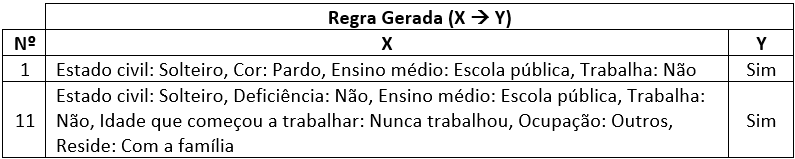
\includegraphics[scale=0.75]{Figuras/Suporte_30_atributos_22.png}
	\end{center}
\end{table}


\par
\textcolor{red}{Avaliando os testes com 25\% de suporte mínimo, foram geradas regras para as bases com 9 e 22 atributos e para a base com 4 atributos nenhuma regra foi obtida. Analisando a única regra que foi gerada para a base com 9 atributos, diz que 2\% dos candidatos que eram aprovados (197 instancias), eles não trabalhavam, não possuíam algum tipo de deficiência e o meio de transporte utilizado era o coletivo, representado na Tabela 5.Já para a primeira regra gerada para a base com 22 atributos, 2\% dos candidatos que foram aprovados (197 instancias) eram solteiros, sustentados pela família e utilizava o transporte coletivo, como representado na Tabela 6.}

\par
\begin{table}[!htp]
	\begin{center}
    \caption{\label{fig:waveform_fig} Suporte Mínimo 25\% e Confiança Mínima 70\% para a base com 9 atributos.}
	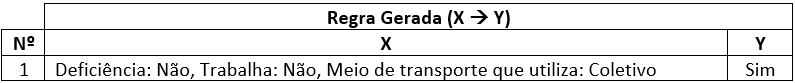
\includegraphics[scale=0.75]{Figuras/Suporte_25_atributos_9.png}
	\end{center}
\end{table}

\par
\begin{table}[!htp]
	\begin{center}
    \caption{\label{fig:waveform_fig} Suporte Mínimo 25\% e Confiança Mínima 70\% para a base com 22 atributos.}
	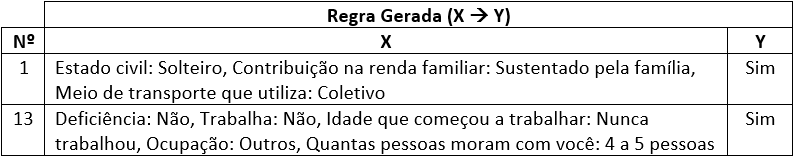
\includegraphics[scale=0.75]{Figuras/Suporte_25_atributos_22.png}
	\end{center}
\end{table}

\par
\textcolor{red}{Com o suporte mínimo de 15\%, as bases de dados com 4 e 9 atributos obtiveram somente uma regra gerada, enquanto, para a base de dados com 22 atributos, foi obtido 67 regras geradas, sendo que é considerada a maior quantidade de regras que já foi gerada para todos os suportes mínimos testados. Começando com a regra gerada para a base com 4 atributos, como demonstrado na Tabela 7, indica que os candidatos que tem uma mãe com ensino médio completo e possui de 4 a 5 pessoas morando com eles, influenciam para que eles sejam aprovados.}

\par
\begin{table}[!htp]
	\begin{center}
    \caption{\label{fig:waveform_fig} Suporte Mínimo 15\% e Confiança Mínima 70\% para a base com 4 atributos.}
	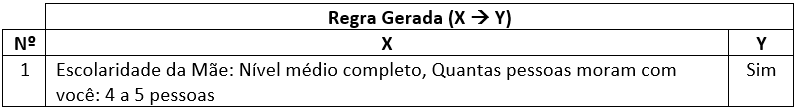
\includegraphics[scale=0.75]{Figuras/Suporte_15_atributos_4.png}
	\end{center}
\end{table}

\par
\textcolor{red}{Já para a base com 9 atributos, a regra gerada indica que os candidatos que possuem um pai que é servidor público, mora com a família e possui de 4 a 5 pessoas morando com eles, são aprovados no vestibular, como apresentado na Tabela 8.}

\par
\begin{table}[!htp]
	\begin{center}
    \caption{\label{fig:waveform_fig} Suporte Mínimo 15\% e Confiança Mínima 70\% para a base com 9 atributos.}
	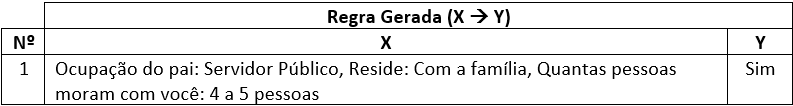
\includegraphics[scale=0.75]{Figuras/Suporte_15_atributos_9.png}
	\end{center}
\end{table}

\par
\textcolor{red}{Para a base de dados com 22 atributos com um suporte mínimo de 15\%, conforme é demonstrado da Tabela 9, na primeira regra gerada, a idade de 18 a 21 anos e a mãe como principal responsável, influenciavam para que o candidato fosse aprovado, enquanto para a última regra gerada, os candidatos que eram pardos, que não frequentavam cursinho pré-vestibular, nunca trabalharam e moravam com a família, eles eram aprovados. As regras geradas paras as bases com 4, 9 e 22 atributos, com um suporte de 15\%, influenciavam 1,4\% dos candidatos (118 instancias).}

\par
\begin{table}[!htp]
	\begin{center}
    \caption{\label{fig:waveform_fig} Suporte Mínimo 15\% e Confiança Mínima 70\% para a base com 22 atributos.}
	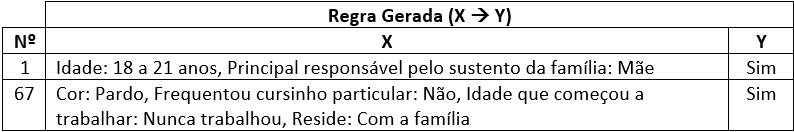
\includegraphics[scale=0.75]{Figuras/Suporte_15_atributos_22.png}
	\end{center}
\end{table}



\subsection{Regras geradas para os candidatos que não foram aprovados}


\par
\textcolor{red}{Para os testes com a base de dados dos candidatos que não foram aprovados, dos 4 suportes mínimos utilizados, apenas 3 geraram regras para as bases de dados, que foram os suportes de 30\%, 25\% e 15\%, sendo que para os suportes testados, geraram regras somente para a base com 22 atributos. Começando com o suporte mínimo de 30\%, como podemos ver na Tabela 10, foi gerado apenas uma regra associada a variável de Aprovados, indicando que que 27\% dos candidatos (2.335 instancias) que não foram aprovados eles eram solteiros, com o tom de pele pardo, não trabalhavam e possuíam residência própria.}


\par
\begin{table}[!htp]
	\begin{center}
    \caption{\label{fig:waveform_fig} Suporte Mínimo 30\% e Confiança Mínima 70\% para a base com 22 atributos.}
	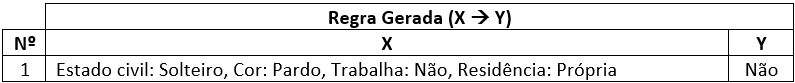
\includegraphics[scale=0.75]{Figuras/Suporte_30_Nao_atributos_22.png}
	\end{center}
\end{table}

\par
\textcolor{red}{Semelhante ao anterior, o suporte mínimo de 25\% gerou uma única regra, somente para a base de 22 atributos, como demonstrado na Tabela 11, a regra gerada indica que 22\% dos candidatos que não foram aprovados (1.946 instancias), eram solteiros, possuem uma renda mensal familiar de 2 a 4 salários mínimos, a residência deles é própria e moram com a família.}

\par
\begin{table}[!htp]
	\begin{center}
    \caption{\label{fig:waveform_fig} Suporte Mínimo 25\% e Confiança Mínima 70\% para a base com 22 atributos.}
	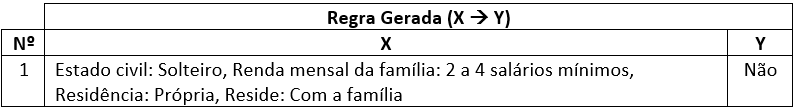
\includegraphics[scale=0.75]{Figuras/Suporte_25_Nao_atributos_22.png}
	\end{center}
\end{table}

\par
\textcolor{red}{Com um suporte mínimo de 15\%, foi obtido regras apenas para a base de dados com 22 atributos, tendo um total de 23 regras geradas. Para a primeira regra, os candidatos que não era deficiente, o ensino médio foi em escola particular e possuía outro tipo de trabalho que não foi mencionado nas opções dadas, eles não eram aprovados. Já para a última regra, para os candidatos com a idade entre 18 a 21 anos, solteiro, não possuía algum tipo de deficiência, o ensino médio foi em escola pública, era sustentado pela família, não trabalhava, possuía uma residência própria e morava com a família, todos esses fatores influenciavam para que eles não fossem aprovados, que era no total de 14\% dos candidatos (1.168 instancias), conforme o que é demonstrado na Tabela 12.}

\par
\begin{table}[!htp]
	\begin{center}
    \caption{\label{fig:waveform_fig} Suporte Mínimo 15\% e Confiança Mínima 70\% para a base com 22 atributos.}
	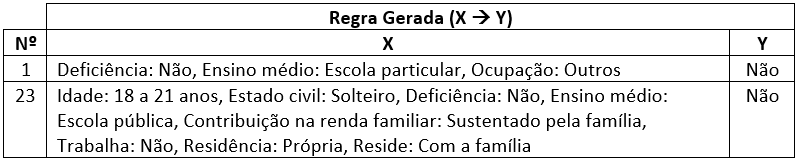
\includegraphics[scale=0.75]{Figuras/Suporte_15_Nao_atributos_22.png}
	\end{center}
\end{table}


\subsection{Observações nas taxas de confiança e lift para os resultados obtidos}

\par
\textcolor{red}{Nos resultado obtidos com o algoritmo de associação, para todos os casos que foram gerados as regras, a porcentagem de confiança de todas essas regras eram de 100\%, o motivo de todas elas possuírem essa taxa, foi pelo fato de que a base teve que ser dividida em duas partes (candidatos aprovados e não aprovados), para poder retirar a tendência  do algoritmo de gerar regras somente para os candidatos que não foram aprovados, que no caso, eram os que possuíam mais registros. Como o algoritmo foi aplicado em uma base onde a variável Aprovado possuía somente uma classe (Sim ou Nao), as regras geradas associadas para essa variável obtiveram resultados com 100\% de confiança, ou seja, a frequência na qual os atributos aparecem em transações que contenham a classe da variável Aprovado é sempre de 100\%, a para as duas bases. }

\par
\textcolor{red}{Comparando com trabalho de \citeonline{LeandroSilva2014} que serviu como base paras os testes deste trabalho, as regras que foram geradas para a sua base, possuíam taxas que variavam de 70\% a 100\% de confiança. O fator principal que influenciava essas porcentagens, foi porque, a variável principal deles a Nota da prova, continha 4 classes que possuíam quantidades de registros que não variavam muito entre elas, não possuíam uma classe que era mais predominante, ao contrario deste trabalho, que uma das classe possuía 10 vezes mais a quantidade de registro do que a outra classe. Para o caso do parâmetro Lift, que é uma métrica que classifica as melhores regras, o algoritmo classificou para todas as regras geradas, associada a variável Aprovado, o valor 1 de importância, ou seja, todas as regras obtidas possuem o mesmo grau de importância.}

\par
\textcolor{red}{Lembrando que outras regras foram geradas para os mesmos casos testados, onde elas possuíam confiança de 80\% a 90\% e lift abaixo e acima do valor 1, contudo, eles não foram mencionados neste trabalho, pelo fato de não serem associados a variável que é importante para esta pesquisa, no caso, a variável Aprovado.}